% ====================================================================
% VİZE RAPOR ŞABLONU – Türk Masalları Derlemesi Web Sayfası
% --------------------------------------------------------------------
% DERLEME: Overleaf'te Menu > Compiler > XeLaTeX (pdfLaTeX de çalışır).
%
% KURALLAR (şablonu kullanmadan önce okuyun):
%  1. Bölüm başlıklarını SİLMEYİN ve sırasını DEĞİŞTİRMEYİN.
%  2. [KÖŞELİ PARANTEZ] içindeki ve gri renkli açıklama metinlerini
%     kendi bilgilerinizle değiştirin; açıklama metinlerini silin.
%  3. MEBİS'e YALNIZCA bu raporun PDF'ini yükleyin.
%     ZIP ve HTML dosyası YÜKLEMEYİN. Tüm kontroller GitHub'dan yapılır.
%  4. Kapaktaki GitHub ve YouTube bağlantıları doğru ve tıklanabilir
%     olmalıdır. Teslimden önce PDF'teki bağlantılara tıklayıp deneyin.
%  5. Haftalık katkı tablosundaki görseller için resim dosyalarını
%     (hafta1.png, hafta2.png, ...) Overleaf projesine yükleyin.
%     Dosya adlarında boşluk ve Türkçe karakter kullanmayın.
%     Resim yoksa tabloda "görsel ekleyin" kutusu görünür.
%  6. Yapay zekâ kullandıysanız Bölüm 5'i doldurun.
% ====================================================================
\documentclass[12pt,a4paper]{article}

\usepackage{iftex}
\ifPDFTeX
  \usepackage[T1]{fontenc}
  \usepackage[utf8]{inputenc}
\else
  \usepackage{fontspec}
\fi
\usepackage[turkish]{babel}
\usepackage[margin=2.4cm]{geometry}
\usepackage{setspace}
\usepackage{graphicx}
\usepackage{booktabs}
\usepackage{longtable}
\usepackage{array}
\usepackage{colortbl}
\usepackage{xcolor}
\usepackage{enumitem}
\usepackage{listings}
\usepackage{amssymb}
\usepackage{caption}
\usepackage{fancyhdr}
\usepackage{hyperref}

\onehalfspacing
\setlength{\parindent}{0pt}
\setlength{\parskip}{6pt}
\setlist{itemsep=2pt, topsep=4pt}
\hypersetup{colorlinks=true, linkcolor=blue!50!black, urlcolor=blue!50!black}

\definecolor{ana}{HTML}{14325C}
\definecolor{acik}{HTML}{EEF2F8}

\lstset{basicstyle=\ttfamily\small, backgroundcolor=\color{acik},
  frame=single, rulecolor=\color{ana}, breaklines=true,
  columns=fullflexible, keepspaces=true, showstringspaces=false,
  literate={ü}{{\"u}}1 {Ü}{{\"U}}1 {ı}{{\i}}1 {İ}{{\.I}}1
           {ş}{{\c{s}}}1 {Ş}{{\c{S}}}1 {ğ}{{\u{g}}}1 {Ğ}{{\u{G}}}1
           {ö}{{\"o}}1 {Ö}{{\"O}}1 {ç}{{\c{c}}}1 {Ç}{{\c{C}}}1}

\pagestyle{fancy}
\setlength{\headheight}{15pt}
\fancyhf{}
\fancyhead[L]{MASALNAME: Kaybolan Hikâyeler Atlası}
\fancyhead[R]{Vize Raporu}
\fancyfoot[C]{\thepage}

% ---------- Yardımcı komutlar ----------
% Gri açıklama metni (silinecek yönergeler için)
\newcommand{\aciklama}[1]{{\color{gray}\itshape (#1)}}

% Haftalık tablo görseli: dosya yoksa "görsel ekleyin" kutusu çıkar
\newcommand{\haftagorsel}[2]{%
  \IfFileExists{#1}{%
    {\shorthandoff{=}\includegraphics[width=\linewidth,height=4.2cm,keepaspectratio]{#1}}%
  }{%
    \fbox{\parbox[c][2.6cm][c]{\dimexpr\linewidth-2\fboxsep-2\fboxrule\relax}{%
      \centering\small\color{gray} Ekran görüntüsü / görsel ekleyin\\ \texttt{#1}}}%
  }%
}
% Haftalık katılım kutuları (işaretlemek için $\square$ yerine $\boxtimes$ yazın)
\newcommand{\katilimderste}{\par\vspace{3pt}\small $\boxtimes$ Ders içinde katılım sergiledim\par $\square$ Telafi yaptım}
\newcommand{\katilimtelif}{\par\vspace{3pt}\small $\square$ Ders içinde katılım sergiledim\par $\boxtimes$ Telafi yaptım}
\newcommand{\katilimsonra}{\par\vspace{3pt}\small $\square$ Ders içinde katılım sergiledim\par $\square$ Telafi yaptım}

% Ek görsel: dosya yoksa hiçbir şey göstermez
\newcommand{\haftaek}[1]{%
  \IfFileExists{#1}{\\[4pt]{\shorthandoff{=}\includegraphics[width=\linewidth,height=4.2cm,keepaspectratio]{#1}}}{}%
}

% ---------- Kapak bilgileri ----------
\newcommand{\universite}{İstanbul Medipol Üniversitesi / Görsel İletişim Tasarımı}
\newcommand{\dersadi}{Programlamaya Giriş}
\newcommand{\hocaadi}{Meral Şentürk}
\newcommand{\ogrenciadi}{Nida Tecirlioğlu}
\newcommand{\ogrencino}{86230005}
\newcommand{\projeadi}{MASALNAME: Kaybolan Hikâyeler Atlası}
% Bağlantıları tam adres olarak yazın (https:// ile başlayarak)
\newcommand{\githublink}{\url{https://github.com/nidatecirli/masalname}}
\newcommand{\youtubelink}{\textcolor{red!70!black}{Video bağlantısı henüz eklenmedi}}

\begin{document}

% ====================================================================
% KAPAK
% ====================================================================
\begin{titlepage}
\centering
\vspace*{0.5cm}
{\large \universite \par}
\vspace{1.1cm}
{\Huge\bfseries\color{ana} \projeadi \par}
\vspace{0.4cm}
{\Large Türk Masalları Derlemesi Web Sayfası \par}
{\large Vize Raporu \par}
\vspace{1.1cm}
{\large \textbf{Ders:} \dersadi \par}
{\large \textbf{Öğretim Üyesi:} \hocaadi \par}
\vspace{0.7cm}
{\large \textbf{Hazırlayan:} \ogrenciadi \par}
{\large \textbf{Öğrenci No:} \ogrencino \par}
\vspace{0.55cm}
{\small\color{red!70!black}Sunum videosu henüz kaydedilmedi. Haftalık tarihler ekran görüntülerinden doğrulanamadığı için kesin tarih yazılmadı; katılım/telafi bilgileri öğrencinin beyanına göre işaretlendi.\par}
\vspace{0.4cm}
\fbox{\parbox{0.88\linewidth}{\centering\vspace{6pt}
{\large\bfseries Proje Bağlantıları}\\[8pt]
\textbf{GitHub deposu:}\\ \githublink \\[8pt]
\textbf{YouTube sunum videosu:}\\ \youtubelink
\vspace{6pt}}}
\vfill
{\large 29 Ekim 2026 \par}
\end{titlepage}

\tableofcontents
\newpage

% ====================================================================
\section{Giriş}
% ====================================================================
MASALNAME, Türk halk anlatılarını deneysel ve etkileşimli bir dijital atlas içinde sunmak amacıyla geliştirilmiştir. Projede, farklı olay örgülerine ve anlatı türlerine sahip 12 masal kısa yeniden anlatımlar biçiminde bir araya getirilmiştir. Sayfanın görsel dili gece gökyüzü, yıldızlar ve masal kapıları fikrinden hareketle oluşturulmuştur. Web sayfası tek bir HTML dosyası olarak hazırlanmış; CSS kodları \texttt{<style>} ve JavaScript kodları \texttt{<script>} etiketi içinde tutulmuştur. Harita, arama, tür filtreleri, okuma penceresi, ruh hâline göre masal keşfi, favoriler ve okuma pasaportu JavaScript ile çalışır. Tasarımda hazır bir web sitesi teması kullanılmamış; görsel hiyerarşi ve etkileşim akışı proje gereksinimlerine göre oluşturulmuştur. Bu rapor masalların seçimini, tasarım kararlarını, kodun temel çalışma mantığını, yapay zekâ kullanımını ve test sürecini açıklar.

\subsection{Proje Özeti}
MASALNAME, kullanıcıyı klasik bir masal listesinden çok yıldız haritası üzerinden keşfe davet eden tek sayfalı bir web deneyimidir. Ana ekranda büyülü bir portal ve giriş metni bulunur; yıldız haritasındaki her düğme ilgili masalın okuma penceresini açar. Arşiv alanında başlık, açıklama ve masal metni üzerinden arama yapılabilir; masallar türlerine göre süzülebilir. Kullanıcı ruh hâline göre öneri alabilir, günün masalına geçebilir, masalları favorilerine ekleyebilir ve okuduklarını pasaportunda işaretleyebilir. CSS ve JavaScript aynı HTML dosyasında bulunduğu için proje harici kütüphanelere veya dış görsel dosyalarına bağlı değildir.

\subsection{Gereksinimlerin Karşılanması}
\begin{center}
\rowcolors{2}{acik}{white}
\begin{tabular}{@{}p{8.2cm}c@{}}
\toprule
\rowcolor{ana}\textcolor{white}{\textbf{Gereksinim}} & \textcolor{white}{\textbf{Durum}} \\
\midrule
Masal sayısı 8--12 arasında (12 masal)             & $\boxtimes$ \\
Tek HTML dosyası                                    & $\boxtimes$ \\
Stil kodları içsel (\texttt{<style>} içinde)        & $\boxtimes$ \\
Betik kodları içsel (\texttt{<script>} içinde)      & $\boxtimes$ \\
İnternetsiz açılıp çalışıyor                        & $\boxtimes$ \\
JavaScript sayfada anlamlı bir işlev görüyor        & $\boxtimes$ \\
Masal metinleri kendi cümlelerimle yazıldı          & $\boxtimes$ \\
Sayfa telefonda da düzgün görünüyor                 & $\boxtimes$ \\
\bottomrule
\end{tabular}
\end{center}
Not: Öğrenci, 12 masalın metinlerini kendi cümleleriyle yazdığını belirtmiştir. Kaynaklar masal başlıkları ve yazar/derleyen bilgilerinin izlenebilmesi için listelenmiştir; metinler doğrudan kopya olarak sunulmamıştır. Masaüstü ve mobil görünüm için kullanıcı tarafından sağlanan güncel ekran görüntüleri Bölüm 3.4’e eklenmiştir.

% ====================================================================
\section{Masalların Seçimi}
% ====================================================================
Masallar, anlatı çeşitliliği, karakterlerin farklılığı ve sundukları davranışsal ya da duygusal temalar dikkate alınarak seçilmiştir. Derlemede zekâ ve problem çözme, dayanışma, iyilik, dönüşüm, fırsat ve macera gibi farklı temalar yer alır. Bu çeşitlilik kullanıcının birden fazla anlatı türü arasında gezinmesine ve kendisine yakın bir hikâyeyi seçmesine olanak verir. Yazar/derleyen bilgileri, sağlanan Türk Masal Külliyatı I PDF dosyalarında belirtildiği biçimde aktarılmıştır.

\begin{longtable}{@{}cp{4cm}p{3cm}p{5.4cm}@{}}
\toprule
\textbf{No} & \textbf{Masal} & \textbf{Tür} & \textbf{Seçilme nedeni} \\
\midrule
\endhead
1 & Yalancı ile Padişah & Zekâ & Söz oyunları ve akıl yoluyla çözüm üretme temasını temsil eder. \\
2 & Ayı ve Yavru Enik & Zekâ & Korku karşısında soğukkanlılık ve pratik düşünmeyi işler. \\
3 & Balıkçı ile Deniz Kızı & Dönüşüm & Hırs, isteklerin sınırı ve sahip olduklarının değerini anlatır. \\
4 & Kurt, Kuş ve Sincap & Dayanışma & Farklı karakterlerin ortak bir sorun için birlikte çalışmasını gösterir. \\
5 & Üç Şaka & Zekâ & Şaka, dikkat ve söylenen sözleri sorgulama temalarını içerir. \\
6 & Akıllı Ormancı & Zekâ & Güç ile akıl arasındaki farkı anlaşılır bir olayla sunar. \\
7 & Kaplumbağa ile Tilki & Zekâ & Hileye karşı sabır ve yaratıcı problem çözmeyi vurgular. \\
8 & Yoksul Kunduracı & İyilik & Karşılık beklemeden yardım etme ve minnettarlık temasını taşır. \\
9 & İnatçı Keçi & Dönüşüm & Uyarıları dinleme ve davranışını gözden geçirme fikrini işler. \\
10 & Aklı Kıt Adam & Fırsat & Fırsatları fark etme ve kararların sonuçlarını değerlendirme temasını işler. \\
11 & Vur Tokmağım Vur & Macera & Olağanüstü armağanlar ve bunların doğurduğu sonuçlarla ilerler. \\
12 & Hazinenin Kapısını Açan Mercimek Çocuk & Macera & Küçük olmanın yetenek ve cesarete engel olmadığını gösterir. \\
\bottomrule
\end{longtable}

% ====================================================================
\section{Tasarım Kararları}
% ====================================================================
Tasarım, hazır bir web sitesi teması kopyalamak yerine MASALNAME için oluşturulan görsel sistem ve kullanıcı akışı üzerine kurulmuştur. Arayüzün ana metaforu, her yıldızın bir masal kapısını temsil ettiği bir gece atlasıdır. Bu yaklaşım hem masal temasını destekler hem de kullanıcıya sayfayı sırayla okumak yerine keşfetme olanağı verir.

\subsection{Konuya Uygunluk}
Görsel dil, masalların gizemli ve hayal gücüne açık atmosferini yansıtmak için gece gökyüzü, ışıklı yıldızlar, yörüngeler ve portal biçimlerinden yararlanır. Koyu lacivert-mor zemin, sahneye derinlik verirken altın rengi ana yönlendirmeleri ve masal kapılarını öne çıkarır. Pembe ve nane tonları duygusal vurgu ve durum işaretleri olarak kullanılır. Başlıklarda Georgia benzeri serif yazı tipi anlatıya editoryal ve masalsı bir ton kazandırır; küçük arayüz etiketlerinde Arial/Helvetica benzeri sans-serif yazı tipi okunabilirliği artırır.

\subsection{Renk Paleti ve Yazı Tipi}
\begin{center}
\rowcolors{2}{acik}{white}
\begin{tabular}{@{}llp{6.4cm}@{}}
\toprule
\rowcolor{ana}\textcolor{white}{\textbf{Ad}} & \textcolor{white}{\textbf{Kod}} & \textcolor{white}{\textbf{Nerede / neden kullandınız?}} \\
\midrule
Gece laciverdi & \texttt{\#0B0B20} & Ana arka plan; gece ve gizem atmosferi oluşturur. \\
Altın & \texttt{\#F3D47B} & Portal, yıldız ve ana eylemlerde vurgu rengi. \\
Pembe / nane / lila & \texttt{\#F18AB2} / \texttt{\#A2E9DD} / \texttt{\#C9B8FF} & Duygusal vurgu, ikincil işaretler ve harita ayrıntıları. \\
Serif / sans-serif & -- & Büyük başlıklarda Georgia; arayüz metinlerinde Arial/Helvetica sistem yazı tipleri. \\
\bottomrule
\end{tabular}
\end{center}

\subsection{Okunabilirlik, Gezinme ve Duyarlı Tasarım}
\begin{itemize}
  \item \textbf{Okunabilirlik:} Okuma penceresinde ayrı bir metin alanı, rahat satır aralığı, yazı boyutunu artırıp azaltma düğmeleri ve ilerleme çizgisi bulunur. Koyu arka plan ile açık metin arasında yüksek karşıtlık kurulmuştur.
  \item \textbf{Gezinme:} Ana menü, yıldız haritası, arama alanı, tür filtreleri, rastgele masal düğmesi ve günün masalı bağlantısı farklı giriş yolları sunar.
  \item \textbf{Duyarlı tasarım:} CSS medya sorguları geniş ekranda yan yana yerleşimi; dar ekranda tek sütun ya da iki sütunlu kartları ve açılır menüyü kullanır.
  \item \textbf{Tutarlılık:} Aynı renk paleti, dairesel motifler, yıldız sembolleri ve serif başlıklar sayfa bölümleri boyunca tekrar eder.
\end{itemize}

\subsection{Ekran Görüntüleri}
Aşağıdaki görseller, GitHub Pages üzerinde yayımlanan MASALNAME'nin masaüstü ve mobil arayüzünden alınmıştır. Masaüstü görselleri açılış portalını ve yıldız haritasını; mobil görselleri ise açılış alanı ile masal kartlarının dar ekranda nasıl yerleştiğini gösterir.
\begin{center}
\begin{minipage}[t]{0.49\textwidth}
  \centering
  {\shorthandoff{=}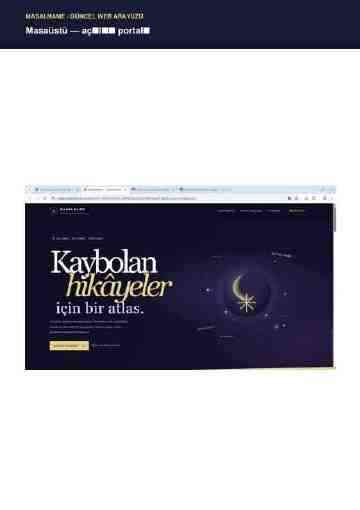
\includegraphics[width=\linewidth,height=4.3cm,keepaspectratio]{assets/site-01.jpg}}\\[3pt]
  {\small\emph{Masaüstü: açılış portalı}}
\end{minipage}\hfill
\begin{minipage}[t]{0.49\textwidth}
  \centering
  {\shorthandoff{=}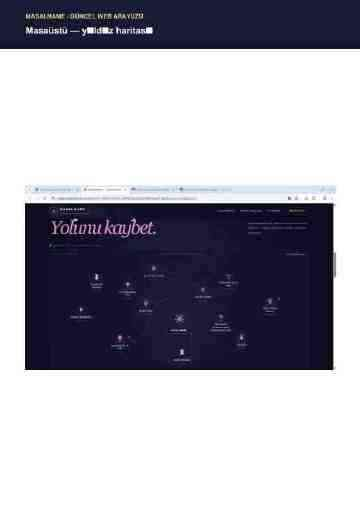
\includegraphics[width=\linewidth,height=4.3cm,keepaspectratio]{assets/site-02.jpg}}\\[3pt]
  {\small\emph{Masaüstü: yıldız haritası}}
\end{minipage}

\vspace{0.45cm}

\begin{minipage}[t]{0.40\textwidth}
  \centering
  {\shorthandoff{=}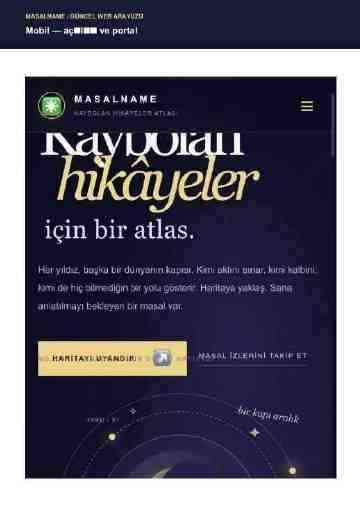
\includegraphics[width=\linewidth,height=5.2cm,keepaspectratio]{assets/site-03.jpg}}\\[3pt]
  {\small\emph{Mobil: arama ve masal kartları}}
\end{minipage}\hfill
\begin{minipage}[t]{0.40\textwidth}
  \centering
  {\shorthandoff{=}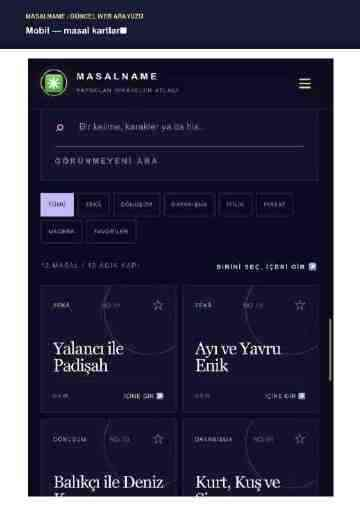
\includegraphics[width=\linewidth,height=5.2cm,keepaspectratio]{assets/site-04.jpg}}\\[3pt]
  {\small\emph{Mobil: günlük masal alanı}}
\end{minipage}
\end{center}

% ====================================================================
\section{Gerçekleştirme}
% ====================================================================
Bu bölüm, sayfanın temel teknik kararlarını ve kullanıcı etkileşimlerinin nasıl çalıştığını açıklar. Kod örnekleri, uygulamadaki daha geniş işlevlerin kısa parçalarıdır.

\subsection{HTML Yapısı}
Belge \texttt{<!doctype html>} bildirimiyle başlar ve Türkçe içerik için \texttt{lang="tr"} kullanır. \texttt{<head>} içinde karakter kodlaması, mobil görünüm için viewport, tema rengi ve açıklama bilgileri yer alır. \texttt{<body>} içinde üst gezinme alanı, açılış bölümü, yıldız haritası, ruh hâli seçimi, masal pasaportu, arşiv, günlük masal, kaynakça ve alt bilgi bulunur. Okuma alanı, sayfadan ayrılmadan açılan bir iletişim penceresi (modal) olarak hazırlanmıştır. Masal verileri tek bir JavaScript dizisinde tutulur; harita düğmeleri ve kartlar bu verilerden üretilir.

\subsection{İçsel CSS}
CSS kodu aynı dosyada \texttt{<style>} etiketinde bulunur. \texttt{:root} içinde renk değişkenleri tanımlanır; böylece ana palet tek noktadan yönetilir. Grid ve Flexbox yerleşimleri, kartlar, portal, okuma penceresi ve pasaport bölümü için kullanılır. \texttt{@media} kuralları dar ekranlarda menüyü açılır hâle getirir, harita düğmelerini liste düzenine geçirir ve kartların kolon sayısını azaltır. \texttt{prefers-reduced-motion} kuralı, hareket azaltma tercihi bulunan kullanıcılar için animasyonları sınırlar.

\begin{lstlisting}[caption={İçsel CSS'ten önemli bir bölüm}]
/* Core palette and responsive typography */
:root {
  --night: #0b0b20;
  --gold: #f3d47b;
  --pink: #f18ab2;
  --mint: #a2e9dd;
  --lilac: #c9b8ff;
}
@media (max-width: 650px) {
  .mood-choices { grid-template-columns: repeat(2, minmax(0, 1fr)); }
}
\end{lstlisting}

\subsection{İçsel JavaScript}
Masalların her biri \texttt{id}, \texttt{title}, \texttt{type}, \texttt{symbol}, \texttt{desc}, \texttt{minutes} ve \texttt{text} alanlarıyla JavaScript dizisinde tutulur. \texttt{buildMap()} haritadaki düğmeleri oluşturur; \texttt{getVisible()} arama metni ile seçili kategoriye göre sonuçları süzer; \texttt{renderArchive()} kartları ve sonuç sayısını yeniler. \texttt{openStory()} okuma penceresini açar, \texttt{showStory()} seçilen masalın metnini ve gezinme düğmelerini günceller. Favoriler ve okunan masallar tarayıcının \texttt{localStorage} alanında JSON dizileri olarak saklanır. Ruh hâli önerisi, günün masalı ve rastgele seçim de aynı masal dizisinden bir kayıt seçerek okuma penceresini açar.

\begin{lstlisting}[caption={İçsel JavaScript'ten önemli bir bölüm}]
function getVisible() {
  const q = search.value.trim().toLocaleLowerCase("tr");
  return stories.filter(function (s) {
    const matchesType = activeFilter === "Tümü" ||
      (activeFilter === "Favoriler" ? favorites.has(s.id) : s.type === activeFilter);
    const text = [s.title, s.desc, s.type].concat(s.text)
      .join(" ").toLocaleLowerCase("tr");
    return matchesType && text.includes(q);
  });
}
\end{lstlisting}

\subsection{Sayfanın Özellikleri}
\begin{itemize}
  \item \textbf{Yıldız haritası:} Her yıldız düğmesi bir masalı açar; düğmeler aynı veri dizisinden üretilir.
  \item \textbf{Arama ve filtreleme:} Başlık, tür, açıklama ve masal metinleri içinde arama yapılır; türler ve favoriler filtrelenebilir.
  \item \textbf{Okuma penceresi:} Masal metnini açar; yazı boyutu, okuma ilerlemesi, önceki/sonraki masal ve Escape ile kapatma desteği sağlar.
  \item \textbf{Ruh hâliyle keşif:} Seçilen duyguya göre önceden eşleştirilen masallardan biri önerilir.
  \item \textbf{Favoriler:} Kullanıcı yıldız simgesiyle bir masalı kaydedebilir ve Favoriler filtresinden tekrar bulabilir.
  \item \textbf{Masal pasaportu:} Okunan masallar işaretlenir; sayaç ve ilerleme çubuğu güncellenir.
  \item \textbf{Günün masalı ve rastgele seçim:} Kullanıcıya yeni bir hikâyeye ulaşmak için iki farklı yol sunar.
  \item \textbf{Çevrimdışı kullanım:} CSS, JavaScript, dekoratif SVG ve simgeler dosyanın içine gömülüdür; dış kaynak veya kütüphane yüklenmez. Favori ve okuma kayıtlarının kalıcılığı tarayıcı depolama desteğine bağlıdır.
\end{itemize}

% ====================================================================
\section{Yapay Zekâ Kullanımı}
% ====================================================================
Yapay zekâ desteğinden HTML, CSS ve JavaScript geliştirme, etkileşim fikirlerini uygulama, hata ayıklama ve rapor metnini düzenleme süreçlerinde yararlanılmıştır. Öğrenci, 12 masalın metinlerini kendi cümleleriyle yazmıştır; bu nedenle masal metinleri yapay zekâ tarafından yazılmış içerik olarak gösterilmemiştir. Aşağıdaki tablo kullanılan desteğin amacını ve sayfadaki yerini özetler. Görsel üretimi için harici bir görsel dosyası kullanılmamıştır; portal ve dekoratif öğeler CSS, metin simgeleri ve satır içi SVG ile oluşturulmuştur. Kodun çalışma mantığını anlama, test etme ve sunumda açıklama sorumluluğu proje sahibine aittir.

\begin{longtable}{@{}p{2.6cm}p{3.6cm}p{4.2cm}p{3.4cm}@{}}
\toprule
\textbf{Araç} & \textbf{Ne için kullandınız?} & \textbf{İstem (prompt) özeti} & \textbf{Sayfada nerede?} \\
\midrule
\endhead
ChatGPT & HTML / CSS / JavaScript & Tek dosyada, koyu ve deneysel bir masal atlası; arama, filtre, harita ve okuma penceresi oluşturma. & Web sayfasının genel yapısı ve etkileşimleri. \\
ChatGPT & Etkileşim tasarımı ve hata ayıklama & Ruh hâli seçimi, favoriler, günün masalı ve okuma pasaportu gibi ek işlevleri entegre etme ve kod denetimi. & Yeni özellikler ve yayımlama öncesi JavaScript sözdizimi kontrolü. \\
\bottomrule
\end{longtable}

\subsection{Anladığım ve Kendim Yaptığım Kısımlar}
Tasarım yönünü belirlerken gece gökyüzü, yıldız haritası, portal ve masal kapısı metaforlarını tercih ettim. Koyu lacivert-mor zemini altın, pembe, nane ve lila vurgularıyla birleştirdim; başlık, harita, kartlar ve okuma penceresi arasında aynı görsel dili korumaya çalıştım. Kodun temel mantığı; masal verisinin bir dizide tutulması, arama ve filtrelerin bu veri üzerinde çalışması, seçilen kaydın okuma penceresine aktarılması ve kişisel durumların tarayıcıda saklanması üzerine kuruludur. On iki masal metnini kendi cümlelerimle yazdım; kaynakları masal seçiminde ve yazar/derleyen bilgilerini belirtmek için kullandım. Kod ve rapor düzenleme aşamasında yapay zekâ desteğinden yararlanırken tasarım yönü ve içerik kararlarını gözden geçirdim; sunum öncesinde kodun çalışma mantığını kendi cümlelerimle açıklamaya hazırlanacağım.

% ====================================================================
\section{Haftalık Katkılar}
% ====================================================================
Aşağıdaki açıklamalar Nida Tecirlioğlu tarafından gönderilen ekran görüntülerine göre hazırlanmıştır. Öğrencinin bildirimine göre 1., 2. ve 3. haftalarda derse katılım; 4., 5. ve 6. haftalarda ise iş nedeniyle telafi çalışması yapılmıştır. Kesin haftalık tarihler ekran görüntülerinden doğrulanamadığı için tarih uydurulmamıştır. Bu bölümde, öğrenci tarafından sağlanan ekran görüntüleriyle belgelenen 1--6. haftalardaki çalışmalar özetlenmiştir.

\begin{longtable}{@{}>{\raggedright\arraybackslash}p{1.7cm}%
                    >{\raggedright\arraybackslash}p{6.4cm}%
                    >{\centering\arraybackslash}p{6cm}@{}}
\toprule
\rowcolor{ana}\textcolor{white}{\textbf{Hafta}} & \textcolor{white}{\textbf{Yapılan çalışma}} & \textcolor{white}{\textbf{Görsel}} \\
\midrule
\endfirsthead
\toprule
\rowcolor{ana}\textcolor{white}{\textbf{Hafta}} & \textcolor{white}{\textbf{Yapılan çalışma}} & \textcolor{white}{\textbf{Görsel}} \\
\midrule
\endhead
\bottomrule
\endfoot

\textbf{1. hafta} &
\textbf{Tarih:} paylaşılmadı. HTML belgesinin temel iskeletini oluşturan \texttt{doctype}, \texttt{html}, \texttt{head}, \texttt{title} ve \texttt{body} etiketlerini uygulamalı olarak denedim. WorldWideWeb konulu sayfada başlık, paragraf ve liste elemanlarıyla içerik hiyerarşisi kurdum; HTML Online Viewer’da kod ile önizleme alanını karşılaştırdım.\newline \textbf{Görsel kanıt:} \href{https://github.com/nidatecirli/masalname/blob/main/weekly-submissions/week-01.jpg}{week-01.jpg}\katilimderste &
\haftagorsel{weekly-submissions/week-01.jpg}{1} \\
\midrule
\textbf{2. hafta} &
\textbf{Tarih:} paylaşılmadı. İlk HTML sayfasını geliştirerek içerik hiyerarşisini ve sayfa içi gezinmeyi düzenledim. “KONULAR”, “PROJE ÖZETİ”, “NASIL ÇALIŞIR” ve “NASIL KATKI SAĞLANIR” bölümleri ile bağlantı listesini oluşturdum. İçsel CSS ile sayfa genişliği, boşluk, yazı boyutu, renk ve başlık stillerini değiştirdim.\newline \textbf{Görsel kanıt:} \href{https://github.com/nidatecirli/masalname/blob/main/weekly-submissions/week-02.jpg}{week-02.jpg}\katilimderste &
\haftagorsel{weekly-submissions/week-02.jpg}{2} \\
\midrule
\textbf{3. hafta} &
\textbf{Tarih:} paylaşılmadı. HTML Online Viewer üzerinde başlık ve paragraf hiyerarşisi, bağlantılar, listeler ve içerik bölümleriyle ilgili alıştırmalar yaptım. 3.2, 3.4, 3.5 ve 3.7 etiketli örneklerde kod değişikliklerinin önizlemeye etkisini kontrol ettim; butona basıldığında uyarı veya geri bildirim gösterme örneklerini denedim.\newline \textbf{Görsel kanıt:} \href{https://github.com/nidatecirli/masalname/blob/main/weekly-submissions/week-03.jpg}{week-03.jpg}\katilimderste &
\haftagorsel{weekly-submissions/week-03.jpg}{3} \\
\midrule
\textbf{4. hafta} &
\textbf{Tarih:} paylaşılmadı. 4.1, 4.2 ve 4.3 etiketli örneklerde sayaç değerini artırma/azaltma ve sonucu sayfaya yazdırma üzerine çalıştım. Ayrıca giriş alanından kullanıcı adı okumayı ve bir buton tıklanınca karşılama ya da bilet işlemi geri bildirimi göstermeyi denedim.\newline \textbf{Görsel kanıt:} \href{https://github.com/nidatecirli/masalname/blob/main/weekly-submissions/week-04.jpg}{week-04.jpg}\katilimtelif &
\haftagorsel{weekly-submissions/week-04.jpg}{4} \\
\midrule
\textbf{5. hafta} &
\textbf{Tarih:} paylaşılmadı. Müzik temalı çoktan seçmeli bir yarışmada soru ve seçenekleri JavaScript ile üretmeyi denedim. Kullanıcı yanıtına göre doğru/yanlış geri bildirimi gösterme, skoru güncelleme ve yarışmayı yeniden başlatma akışlarını oluşturdum; ekran görüntülerinde oyun 3/3 skorla tamamlanıyor. Gönderilen 5. hafta kanıt grubunda sayaç ekranı da yer aldığından, özgün görsel grubuyla birlikte korundu.\newline \textbf{Görsel kanıt:} \href{https://github.com/nidatecirli/masalname/blob/main/weekly-submissions/week-05.jpg}{week-05.jpg}\katilimtelif &
\haftagorsel{weekly-submissions/week-05.jpg}{5} \\
\midrule
\textbf{6. hafta} &
\textbf{Görsel kaydı:} 21.10.2026 (ekran görüntüsünde görünen tarih; ders tarihi olduğu doğrulanmadı). CodePen üzerinde NOIR adlı alternatif kültür rehberi için HTML, CSS ve JavaScript panellerini kullanarak gezinme menüsü, giriş başlığı, “Sound / Visual / Play” kartları, etkinlik listesi ve e-posta kayıt alanı tasarladım. Renk paletini değiştiren kontrollerle aynı tasarımın turuncu ve mavi gibi farklı görsel atmosferlerde nasıl çalıştığını denedim.\newline \textbf{Görsel kanıt:} \href{https://github.com/nidatecirli/masalname/blob/main/weekly-submissions/week-06.jpg}{week-06.jpg}\katilimtelif &
\haftagorsel{weekly-submissions/week-06.jpg}{6} \\
\end{longtable}

% ====================================================================
\section{Test ve Değerlendirme}
% ====================================================================
Kullanıcı, canlı sayfadaki temel özelliklerin çalıştığını doğrulamış ve masaüstü Chrome ile mobil Safari görünümlerinden ekran görüntüleri paylaşmıştır. GitHub Actions içinde son sürümün içsel JavaScript sözdizimi kontrolü başarıyla geçmiş, GitHub Pages dağıtımı tamamlanmıştır. Bu kontroller otomatik uçtan uca test anlamına gelmez; tarayıcılar arası ayrıntılı testler ve bütün etkileşimlerin ayrı ayrı mobil denemesi son teslim öncesi tekrar yapılabilir.

\begin{center}
\rowcolors{2}{acik}{white}
\begin{tabular}{@{}p{6cm}p{3.4cm}p{3.4cm}@{}}
\toprule
\rowcolor{ana}\textcolor{white}{\textbf{Özellik}} & \textcolor{white}{\textbf{Bilgisayar}} & \textcolor{white}{\textbf{Telefon}} \\
\midrule
Arama, filtre ve yıldız haritası & Kullanıcı denemesinde çalışıyor & Mobil yerleşim görüntülendi; etkileşim testi tamamlanabilir \\
Okuma penceresi, yazı boyutu, gezinme & Kullanıcı denemesinde çalışıyor & Mobil etkileşimler tekrar kontrol edilebilir \\
Favoriler, ruh hâli, pasaport, günlük masal & Yeni sürümde mevcut; temel akış çalışıyor & Mobilde ayrı ayrı son kontrol önerilir \\
\bottomrule
\end{tabular}
\end{center}

\textbf{Denenen tarayıcılar:} Masaüstü Google Chrome ve mobil Safari ekran görüntüleri sağlandı. Ekran görüntüleri canlı sayfa görünümünü belgelemektedir; ayrıntılı tarayıcılar arası otomatik test yapılmamıştır.

% ====================================================================
\section{Sunum Videosu}
% ====================================================================
\begin{center}
\begin{tabular}{@{}ll@{}}
\textbf{Video süresi:} & Henüz kaydedilmedi (hedef: 12--18 dakika) \\
\textbf{Görünürlük:} & Listelenmemiş ya da herkese açık seçilmelidir \\
\textbf{Bağlantı:} & \youtubelink \\
\end{tabular}
\end{center}

\subsection{Video Kontrol Listesi}
Video henüz yüklenmediği için bu kontrol listesi bilinçli olarak boş bırakılmıştır. Video yayımlandıktan sonra her maddeyi gerçekten kontrol edip işaretleyin.
\begin{itemize}
  \item $\square$ Süre 12--18 dakika aralığında.
  \item $\square$ Sunum boyunca kameram açık, yüzüm görünüyor.
  \item $\square$ Görünürlük \textbf{Listelenmemiş} (ya da Herkese açık); \textbf{Özel} değil.
  \item $\square$ Bağlantıyı gizli pencerede açtım, video oynuyor.
  \item $\square$ YouTube videoyu işlemeyi bitirdi.
  \item $\square$ Videoyu baştan sona izledim; ses ve kamera tüm sunumda var.
  \item $\square$ Kapaktaki bağlantı ile bu bölümdeki bağlantı aynı.
\end{itemize}

% ====================================================================
\section{Sonuç ve Kendi Değerlendirmem}
% ====================================================================


Bu projede HTML, içsel CSS ve JavaScript kullanarak Türk masallarını keşif odaklı bir dijital atlasta bir araya getirdim. Ders alıştırmalarında öğrendiğim temel HTML yapısı, CSS ile içerik düzenleme ve JavaScript olaylarını daha kapsamlı bir sayfada arama, filtre, yıldız haritası ve okuma penceresi gibi işlevlerle kullandım. Koyu gece paleti ve yıldız/portal metaforu masal temasını görsel bir sistem hâline getirirken ruh hâliyle keşif, günün masalı, favoriler ve okuma pasaportu kullanıcıya farklı gezinme yolları sunuyor. Tasarım ve kod geliştirme sırasında yapay zekâ desteğinden yararlandım; masal metinlerini kendi cümlelerimle yazdım. Teslim öncesinde haftalık tarihler ve sunum videosu bağlantısı son kez kontrol edilmelidir.

% ====================================================================
\section{Kaynakça}
% ====================================================================
Masal metinleri, yazar/derleyen atıfları ve teknik açıklamalar için başvurulan kaynaklar aşağıda listelenmiştir. Sağlanan PDF'lerde teyit edilemeyen yayın yılı, yayınevi ve sayfa numarası bilgileri eklenmemiştir. Arayüzde harici stok görsel kullanılmamış; dekoratif harita çizgileri satır içi SVG, simgeler ve CSS ile oluşturulmuştur.

\begin{thebibliography}{9}
\bibitem{akm} Atatürk Kültür Merkezi Başkanlığı. (t.y.). \emph{Türk Masal Külliyatı I}. Kullanılan masal PDF dosyaları. Yıl ve yayın bilgileri sağlanan dosyalarda doğrulanamadığı için belirtilmemiştir.
\bibitem{demir} Demir, N. (t.y.). \emph{Yalancı ile Padişah; Ayı ve Yavru Enik; Balıkçı ile Deniz Kızı; Üç Şaka; Kaplumbağa ile Tilki}. Sağlanan PDF dosyalarındaki yazar atıfları.
\bibitem{sargin} Sargın, M. (t.y.). \emph{Kurt, Kuş ve Sincap}. Sağlanan PDF dosyasındaki yazar atfı.
\bibitem{yardimci} Yardımcı, M. (t.y.). \emph{Akıllı Ormancı}. Sağlanan PDF dosyasındaki yazar atfı.
\bibitem{akcam} Akçam, Y. (t.y.). \emph{Yoksul Kunduracı}. Sağlanan PDF dosyasındaki yazar atfı.
\bibitem{ari} Arı, B. (t.y.). \emph{İnatçı Keçi}. Sağlanan PDF dosyasındaki yazar atfı.
\bibitem{erdogan} Erdoğan, S. (t.y.). \emph{Aklı Kıt Adam}. Sağlanan PDF dosyasındaki yazar atfı.
\bibitem{benekkaya} Benek Kaya, A. (t.y.). \emph{Vur Tokmağım Vur}. Sağlanan PDF dosyasındaki yazar atfı.
\bibitem{yasar} Yaşar, S. (t.y.). \emph{Hazinenin Kapısını Açan Mercimek Çocuk}. Sağlanan PDF dosyasındaki yazar atfı.
\bibitem{mdnhtml} MDN Web Docs. (t.y.). \emph{HTML elements reference}. \url{https://developer.mozilla.org/en-US/docs/Web/HTML/Reference/Elements}. Erişim: 25 Ekim 2026.
\bibitem{mdnmedia} MDN Web Docs. (t.y.). \emph{CSS media queries}. \url{https://developer.mozilla.org/en-US/docs/Web/CSS/Guides/Media_queries}. Erişim: 25 Ekim 2026.
\bibitem{mdnlocal} MDN Web Docs. (t.y.). \emph{Window: localStorage property}. \url{https://developer.mozilla.org/en-US/docs/Web/API/Window/localStorage}. Erişim: 25 Ekim 2026.
\bibitem{githubpages} GitHub Docs. (t.y.). \emph{Deploying your website automatically}. \url{https://docs.github.com/en/get-started/start-your-journey/deploying-your-website-automatically}. Erişim: 25 Ekim 2026.
\end{thebibliography}

% ====================================================================
\appendix
\section{Teslim Kontrol Listesi}
% ====================================================================
Teslim etmeden önce doğru olan maddeleri işaretleyin.
\begin{itemize}
  \item $\square$ MEBİS'e \textbf{yalnızca bu raporun PDF'ini} yükleyeceğim. ZIP ve HTML dosyası yüklemeyeceğim.
  \item $\square$ Öğrenci numarası eklendi ve PDF dosya adı \texttt{OgrenciNo\_AdSoyad\_vize.pdf} biçiminde düzenlendi.
  \item $\square$ Kapaktaki GitHub ve YouTube bağlantıları doğru; PDF'te tıklayıp denedim.
  \item $\square$ GitHub deposunda web sayfası (tek \texttt{.html}), rapor PDF'i, \texttt{.tex} kaynakları ve \texttt{README.md} var.
  \item $\square$ GitHub deposu \textbf{herkese açık} (ya da öğretim üyesine erişim verdim).
  \item $\square$ Çalışmamın son hâli teslim saatinden \textbf{önce} depoya gönderildi (sonraki commitler değerlendirilmez).
  \item $\square$ Sayfa içsel CSS ve içsel JavaScript kullanıyor, harici dosya gerektirmiyor.
  \item $\square$ Hazır taslak kullanmadım; yapay zekâ kullandıysam Bölüm 5'i doldurdum.
  \item $\square$ Çalışmanın mantığını sunumda anlatabilirim.
\end{itemize}

\end{document}
